\section{Method RQ 4s - Mapping abnormal or change events with changepoint detection using Accelerometer, GPS and AHN2 data}\label{rq2c}

Assuming that in the optimal circumstances, someone will walk with a specific speed in a monotonous way and the pavement has a regular surface, the measured acceleration in the z-axis will show a monotonous pattern. An \emph{abnormal} peak in the continuous data will indicate a problem or obstacle in the pavement surface. Next to this, a sudden change in the walking speed of the person, could indicate a disturbance of the walking route. Together, a sudden drop in speed, plus a peak in the z-axis acceleration, could indicate big bumb or obstacle which causes a change in the walking behaviour of the pedestrian. For example, tackling a curb obstacle with the rollator. 

By looking at the changes or anomalies in the time series data of speed, slope and z-axis acceleration measured during a walk and linking them to location trough GPS measurements, the physical obstacles or hindrances can be located. The changes or anomalies in time-serie data can be determined by the change-point package of R containing specialized change-point finding algorithms for detecting multiple change-points within data and a variety of test statistics.~\cite{changepoint2015,  killick2014} A changepoint is the estimation of the point at which the statistical properties(mean or variance) of a sequence of observations changes.

\subsection{The changepoint package}
%the changepoint package and possible methods
The ChangePoint package of Killick et al. 2014 contains functions to detect multiple changes in the mean or the variance of large datasets. First we will explain the concept of change-points and the segment in between. Then, the methods offered by the package will be explained and the possibility to choose different statistical models for penalty fitting. The exact approach of identifying multiple change-points, formulas, methods and references can be found in the report of the changepoint package by Killick et al. 2014~\cite{killick2014}

%changepoints and segments
Having an ordered sequence of data $y_{1:n} = (y_{1}, .... , y_{n})$, a change-point is said to occur within this set when there exists a time, $τ ∈ {1, . . . , n − 1}$, such that the statistical properties of segment ${y_{1}, .... , y_{τ}}$ and segment ${y_{τ+1}, .... , y_{n}}$ are different in some way. Consequently the $m$ change-points will split the data into $m + 1$ segments, with the $i^th$ segment containing data $y_{(τ_{i−1} +1):τ_{i}}$ . Each segment will be summarized by a set of parameters.~\cite{killick2014} Possible is to use the two sides: the change-points $CP_{1:m} = (CP_{1}, .... , CP_{m})$ themselves and the segments $y_{(CP_{i−1} +1):CP_{i}}$ between the change-points. Each, with its own set of parameters. 
The average variance or mean of the segment indicates the homogeneous  characteristics of the dataset, between the change-points. 

%possible methods
The Changepoint package implements three multiple change-point algorithms; Binary Segmentation(BS), Segment Neighbourhoods(SN) and the Pruned Exact Linear Time(PELT). Binary Segmentation is an approximate algorithm and most widely used search method. Segment Neighbourhoods has a long computation time but is more exact. PELT is computationally fast and exact. The number of change-points increases linearly as the data set increases. 
In addition the package provides a variety of test statistics for the penalty type settings, for example: BIC, AIC or Hanan-Quinn. 
The penalty settings are used to prevent the model for over fitting and increases the number of parameters in the model to almost always improve the goodness of fit. The default is using no model and taking all measurements into account. When using Asymptotic penalty, the theoretical type I error (0.05) is used. Also a manual penalty can be set, this can be a numeric value or text giving the formula to use. Available variables are n=length of original data. ~\cite{killick2014}

All the different changepoint detection methods had to be tested to see which model approaches the most plausible result and approaches the truth the best. This was shortly done for all individual dataset. Also the best possible penalty settings are considered when there was over or under fitting. We found big difference in characteristics of the dataset for speed, slope and acceleration. Most often the penalty was set manually to $1.5 * log(n)$ to ignore extreme measurements. 

% When over or under-fitting occurs, we adjusted the penalty. Especially in the speed and slope datasets, over-fitting was a problem. Extreme peaks or graduated steps in the speed are due to measurement errors in the GPS. If a model fits too well, these are taken as truth, the penalty settings can even out those extreme measurements. 
% ### Because of overfitting the model of speed a penatlyt type of BIC AIC or Hanan-Quinn can be chosen to solve the problem of overfitting.
% ##  a penalty term for the number of parameters in the model; the penalty term is larger in BIC than in AIC.
% ##he penalty discourages overfitting (increasing the number of parameters in the model almost always improves the goodness of the fit).
% ## we use an adjusted penalty to overcome the problem of overfitting. The GPS contains abonormal peaks due to measurement errors. If a model is generated that fits too well, these are taken as truth. Using a penalty these extreme measurments are not taken into the analysis. These are plausibly artifacts of the data rather
% ## than true changes in the underlying process. In an effort to remove these seemingly spurious changepoints we can increase the penalty to 
% ## The result seem more plausible. 

\subsection{Routes measured}
For testing if the change-point method is usable for detecting obstacles while walking, several test were walked, during the RollatorLoop 2015.
We used the Garmin Summit for the participants and the Leica system on the Meetrollator. 3 smart phones with the Accelerometer (Physics Toolbox version 1.2.9 were used. Here all the accelerometer measurements failed because or the wrong application version.  See Annex \ref{Afailed} for the measured tracks and the accelerometer output. Eventually, the failed measurement with the Leica system, could be used for analysing speed and slope. But the accelerometer was left out here. Also, half way the route, the Leica system stopped walking. Therefor only half of the route was measured. See figure\ref{leicatracks} for the route.
So, secondly a bike ride was monitored for testing the application settings again, with the Accelerometer (Physics Toolbox version 1.3.7) and the GPS Geotracker Application to record GPS. When this seemed to work, also a walk with the measurement rollator was conducted by the researcher herself. Using the Accelerometer (Physics Toolbox version 1.3.7) and the Garmin Summit. Both tracks are shown in figure \ref{tracks}.

\begin{figure}[hb]
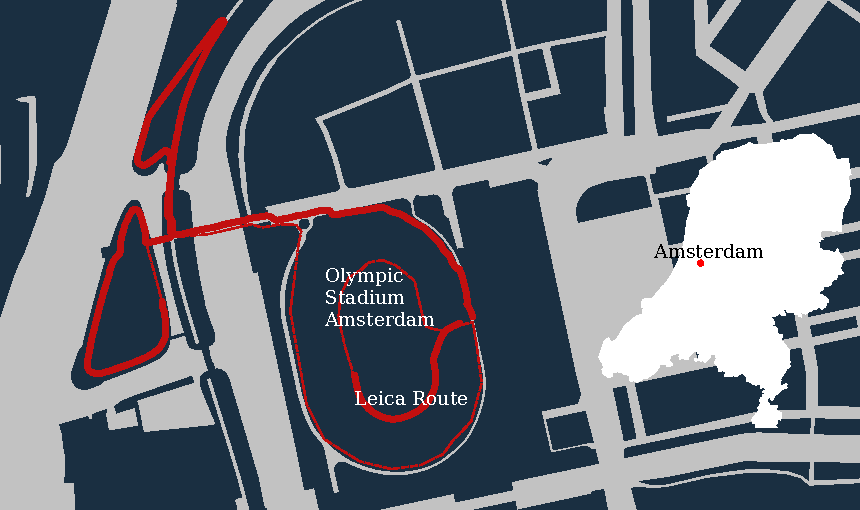
\includegraphics[width=\textwidth]{img/M_overviewRouteLeica.pdf}
\centering
\caption{ Map of Leica route in Amsterdam\label{leicatracks}}
\end{figure}

The datasets of the accelerometer are combined with the location dataset of the GPS measurements. The location assigning is done with the same method as described in the previous section \ref{locationassigning}. Also here the location specific data was added to the dataset, the speed($S$) extracted from the track GPS points and the AHN values, height and slope. Resulting in a feature per observation of:

\begin{equation} 
	F_(i) = [ Time stamp, A_{x}, A_{y}, A_{z}, A_{m}, s, height, slope] 
\end{equation}

The dataset per route was approached as a time-series dataset to applying the changepoint method. Each route and data range on the route had its own specific settings to get the best model of fit. Eventually this resulted in a changepoint feature for every $m^(th)$ changepoint observation:

\begin{equation}
CP_m = [ breakpoint index, mean, variance, time, x,y]
\end{equation}
This is applicable to the acceleration, speed, slope and height. The change-points are detected with the variance setting for the acceleration and mean for change-points detection for speed, height and slope: 

$CP_{mean(s)}, CP_{Var(A_{z})}, CP_{Var(A_{m})}$ and $CP_{mean Height}, CP_{mean slope}$ 

With all change-points having location coordinates($x,y$) in RD new and a time stamp. When plotting all changepoints on the map, visually, patterns in the route can be detected.

\begin{figure}[ht]
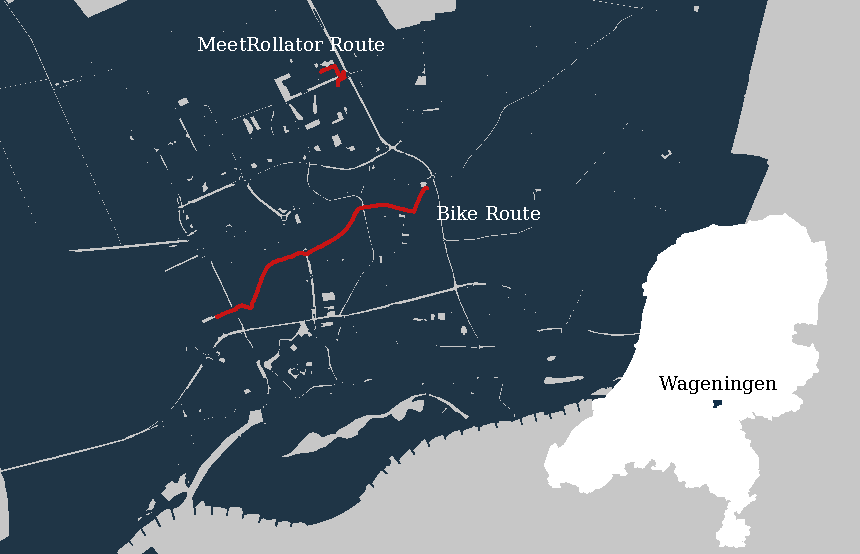
\includegraphics[width=\textwidth]{img/M_overviewRoute.pdf}
\centering
\caption{ Map of tracks measured in Wageningen\label{tracks}}
\end{figure}

